\subsection{Format de sauvegarde d'une scène}

La sauvegarde d’une scène se fera au format XML. La racine scène contiendra une suite d’objets, une lumière et une caméra. Un objet aura pour attribut son format et son répertoire d’accès et sera caractérisé par une translation, une rotation et un redimensionnement. Une lumière sera directionnelle ou ponctuelle et caractérisée par une couleur, une translation et une rotation. La caméra sera caractérisée par une translation, une rotation et un zoom et une ouverture. Le fichier sera validé par un schéma XML tout au long de la phase de développement et lu via des requêtes XPath.

\paragraph{}
Le schéma XML ainsi qu’un fichier XML de test ont été réalisés et sont disponibles en annexe.

\subsection{Test de fluidité}

Le logiciel Meshlab a été utilisé sur différentes machines avec différents modèles 3D pour déterminer un rapport FPS / nombre de points convenable. Les modèles 3D utilisés contiennent entre 40000 et 14 millions de points.

\subsection{Test de portabilité}

Pour s’assurer de la portabilité de QT et OpenGL sur Windows et Linux, un affichage simple d’un modèle 3D dans une fenêtre QT, sans colorations de face, a été fait et testé sur différentes distributions. Les versions 5 de QT et 3.3 d’OpenGL ont été utilisées pour ce prototype et seront utilisées dans la suite du projet. Il a été testé avec des modèles de Stanford comme le dragon, le lapin ou le bouddha.

\subsection{Réduction du nombre de polygones d’un modèle 3D}

Un algorithme permet de réduire le nombre de faces d’un modèle 3D qui en possèderait trop et serait donc impossible à afficher. Il supprime des triangles et fusionne les sommets autour, jusqu’à ce que le nombre de polygones tombe en dessous d’un certain seuil (fig. \ref{fig:poly_reduc}).
\begin{figure}[h]
		\centering
		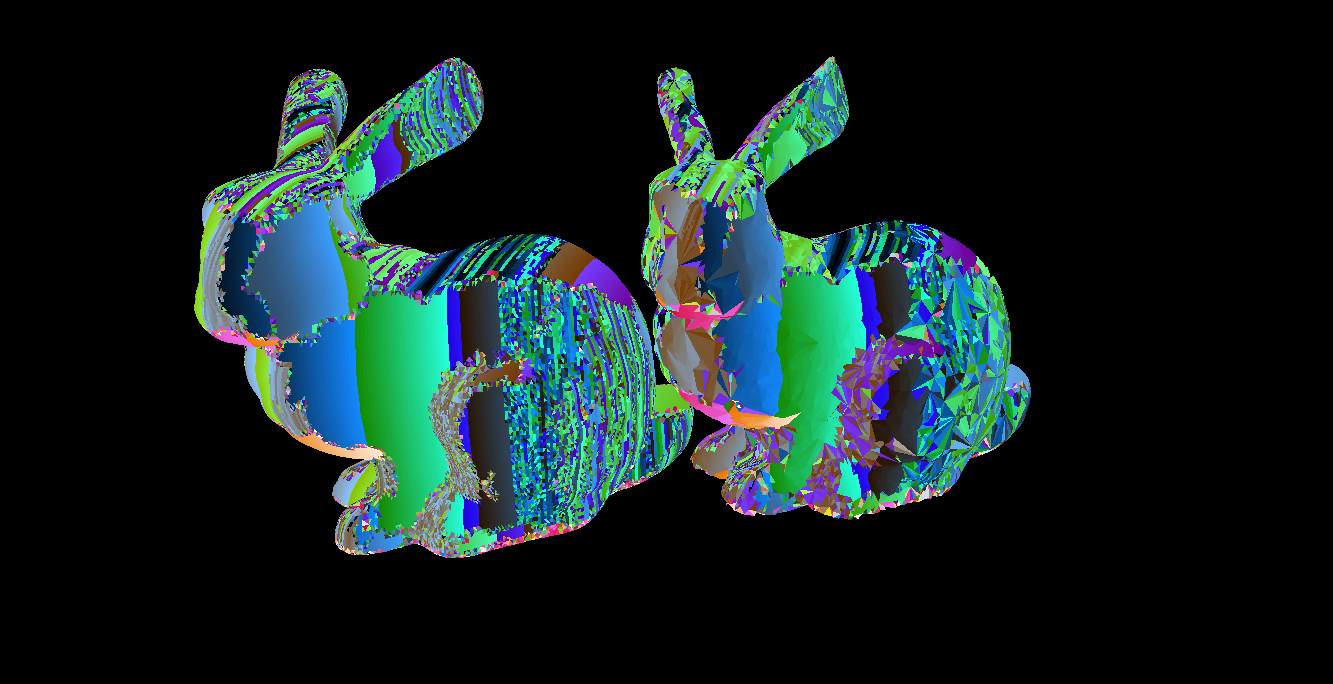
\includegraphics[scale=0.4]{polygon_reduction.png}
		\caption{\label{fig:poly_reduc} \`A gauche modèle 3D d'origine, à droite modèle après suppression de faces }
\end{figure}

\paragraph{}
Ce traitement est effectué lors du chargement et est relativement rapide pour les objets (fig. \ref{fig:poly_reduc_console}).
\begin{figure}[h]
		\centering
		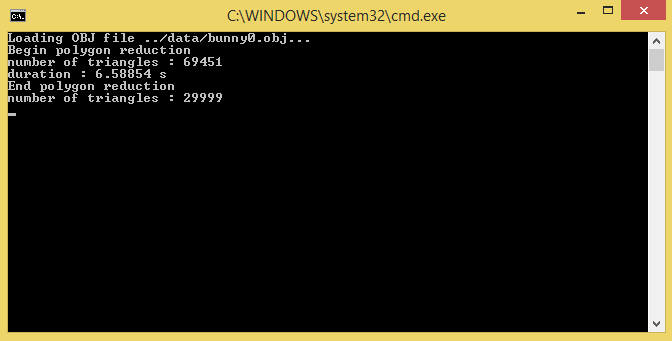
\includegraphics[scale=0.4]{polygon_reduction_console.png}
		\caption{\label{fig:poly_reduc_console}Un test effectué avec l'algorithme sur le modèle de la figure \ref{fig:poly_reduc} montre qu'il met moins de 7 secondes pour supprimer 40000 faces}
\end{figure}